% !TEX encoding = UTF-8 Unicode

\documentclass[a4paper]{article}

\usepackage{color}
\usepackage{url}
\usepackage[T2A]{fontenc} % enable Cyrillic fonts
\usepackage[utf8]{inputenc} % make weird characters work
\usepackage{graphicx}
\graphicspath{ {img/} }

\usepackage[english,serbian]{babel}
%\usepackage[english,serbianc]{babel} %ukljuciti babel sa ovim opcijama, umesto gornjim, ukoliko se koristi cirilica

\usepackage[unicode]{hyperref}
\hypersetup{colorlinks,citecolor=green,filecolor=green,linkcolor=blue,urlcolor=blue}

%\newtheorem{primer}{Пример}[section] %ćirilični primer
\newtheorem{primer}{Primer}[section]

\begin{document}

%\renewcommand{\abstractname}{Apstrakt} %pisace Sazetak ako se ne ukljuci ova naredba

\title{Primena mašinskog učenja u verifikaciji softvera\\ \small{Seminarski rad u okviru kursa\\Metodologija stručnog i naučnog rada\\ Matematički fakultet}}

\author{Nikola Dimitrijević, Rastko Đorđević,\\
 Luka Živanović, Dimitrije Špadijer\\
 nikoladim95@gmail.com, mi14078@alas.matf.bg.ac.rs,\\
  mi14164@alas.matf.bg.ac.rs, mm11021@alas.matf.bg.ac.rs}
%\date{9.~april 2015.}
\vspace*{-3cm}
    {\let\newpage\relax\maketitle}

\abstract{
U ovom tekstu je ukratko prikazana osnovna forma seminarskog rada. Obratite pažnju da je pored ove .pdf datoteke, u prilogu i odgovarajuća .tex datoteka, kao i .bib datoteka korišćena za generisanje literature. Na prvoj strani seminarskog rada su naslov, apstrakt i sadržaj, i to sve mora da stane na prvu stranu! Kako bi Vaš seminarski zadovoljio standarde i očekivanja, koristite uputstva i materijale sa predavanja na temu pisanja seminarskih radova. Ovo je samo šablon koji se odnosi na fizički izgled seminarskog rada (šablon koji \emph{morate} da ispoštujete!) kao i par tehničkih pomoćnih uputstava. Molim Vas da kada budete predavali seminarski rad, imenujete datoteke tako da sadrže temu seminarskog rada, kao i imena i prezimena članova grupe (ili samo temu i prezimena, ukoliko je sa imenima predugačko). Predaja seminarskih radova biće isključivo preko web forme, a NE slanjem mejla.

\tableofcontents

\newpage

\section{Uvod}
\label{sec:uvod}

Ко жели, може да пише рад ћирилицом. У том случају, неопходно је да су инсталирани одговарајући пакети: texlive-fonts-extra, texlive-latex-extra, texlive-lang-cyrillic, texlive-lang-other. \\

Uz sve novouvedene termine u zagradi naglasiti od koje engleske reči termin potiče. Naredni primeri ilustruju način uvođenja enlegskih termina kao i citiranje.

\begin{primer}
Problem zaustavljanja (eng.~{\em halting problem}) je neodlučiv \cite{haltingproblem}.
\end{primer}

\begin{primer}
Za prevođenje programa napisanih u programskom jeziku C može se koristiti GCC kompajler \cite{gcc}.
\end{primer}

\begin{primer}
 Da bi se ispitivala ispravost softvera, najpre je potrebno precizno definisati njegovo ponašanje \cite{laski2009software}. 
\end{primer}

Reference koje se koriste u ovom tekstu zadate su u datoteci {\em seminarski.bib}. Prevođenje u pdf format u Linux okruženju može se uraditi na sledeći način:
\begin{verbatim}
pdflatex TemaImePrezime.tex 
bibtex TemaImePrezime.aux 
pdflatex TemaImePrezime.tex 
pdflatex TemaImePrezime.tex 
\end{verbatim}
Prvo latexovanje je neophodno da bi se generisao {\em .aux} fajl. {\em bibtex} proizvodi odgovarajući {\em .bbl} fajl koji se koristi za generisanje literature. 
Potrebna su dva prolaza (dva puta pdflatex) da bi se reference ubacile u tekst (tj da ne bi ostali znakovi pitanja umesto referenci). Dodavanjem novih referenci potrebno je ponoviti ceo postupak.  


Broj naslova i podnaslova je proizvoljan. Neophodni su samo Uvod i Zaključak. Na poglavlja unutar teksta referisati se po potrebi. 
\begin{primer}
U odeljku \ref{sec:naslov1} precizirani su osnovni pojmovi, dok su zaključci dati u odeljku \ref{sec:zakljucak}.
\end{primer}

Još jednom da napomenem da nema razloga da pišete:
\begin{verbatim}
\v{s} i \v{c} i \'c ...
\end{verbatim}
Možete koristiti srpska slova
\begin{verbatim}
š i č i ć ... 
\end{verbatim}


Ovde pišem uvodni tekst.
Ovde pišem uvodni tekst. 
Ovde pišem uvodni tekst. 
Ovde pišem uvodni tekst. 


\section{Verifikacija softvera}
\label{sec:verifikacija}

\par U savremenom dobu, računari i računarski sistemi predstavlju sastavni deo svakodnevice, kako u privatnom životu, tako i u poslovnom svetu, a i u državnoj administraciji. Zato je od izuzetnog značaja da softver koji se koristi bude pouzdan. Neispravan softver, u zavisnosti od toga gde se koristio i koliko je veliki bio propust, može izazvati male, ali i ogromne probleme sa teškim posledicama (čak i smrtnim). Oblast razvoja softvera koja se bavi proverom ispravnosti softvera, odnosno potvrđivanjem da softver radi u skladu sa zahtevima, naziva se \emph{verifikacija softvera}.

\par Potrebno je precizirati šta se podrazumeva pod ispravnim softverom. Razlikujemo potpuno ispravan i delimično ispravan softver. Softver se smatra potpuno ispravnim ako se zaustavlja za svaki ulaz i na izlazu daje ispravan rezultat, dok se delimično ispravnim softverom smatra onaj koji za ulaz daje ispravan rezultat ako da se zaustavlja, a dozvoljeno je da se za neki ulaz program ne zaustavlja. Ne postoji algoritamski način da se proveri da li se neki program zaustavlja (tzv. Halting problem), pa se često ni ne ispituje potpuna, već samo delimična ispravnost softvera.

\par Postoje dve osnovne vrste verifikacije softvera. To su dinamička i statička verifikacija softvera.

\subsection{Dinamička verifikacija softvera}
\label{subsec:dinamicka}

\par Dinamička verifikacija softvera zasnovana je na tome da se provera ispravnosti softvera vrši tokom njegovog izvršavanja. Najčešće se dinamička verifikacija softvera vrši testiranjem i ti pojmovi se poistovećuju, što nije sasvim ispravno.

\par Testiranje je složen proces koji obuhvata pronalaženje što raznovrsnijeg skupa ulaza, definisanje očekivanih izlaza za svaki od tih ulaza, a zatim izvršavanje programa i provera da li je program za date ulaze vratio odgovarajuće izlaze.

\subsection{Statička verifikacija softvera}
\label{subsec:staticka}

Ovde pišem tekst. 
Ovde pišem tekst. 
Ovde pišem tekst. 
Ovde pišem tekst. 
Ovde pišem tekst. 
Ovde pišem tekst. 

\section{ML, big data, vr, blockchain, IoT, ar, AI}
\label{sec:naslov2}

Ovde pišem tekst. 
Ovde pišem tekst. 
Ovde pišem tekst. 
Ovde pišem tekst. 

\subsection{... podnaslov}
\label{subsec:podnaslovN}

Ovde pišem tekst. 
Ovde pišem tekst. 
Ovde pišem tekst. 
Ovde pišem tekst. 
Ovde pišem tekst. 
Ovde pišem tekst. 

\section{Nase pricice koje smo izabrali}
\label{sec:naslovN}

Ovde pišem tekst. 
Ovde pišem tekst. 
Ovde pišem tekst. 
Ovde pišem tekst. 
Ovde pišem tekst. 

\subsection{Pravljenje skupova treniranja, testiranja i uporedjivanje uspesnosti modela}
\label{subsec:pregled}

%naslov


% uvod
% mozda nista ovde?
% *chapter.+1

Rad \cite{staticFeatures} predlaze resenje za generisanje ulaznih podataka za algoritme masinskog ucenja na osnovu
izvornog koda kako bi se napravio inteligentni metod detekcije gresaka.

Bitno je prvo definisati kakvim tipovima gresaka se posvecuje paznja u okviru metoda.
Iako postoje drukcije greske, vrsena je selekcija prema vaznosti, odnosno prema tome
koliku stetu mogu da uzrokuju i mogucnost da budu detektovane racunarskim alatom. Izabrani tipovi gresaka su:
% moze se navesti iz koje knjige su uzete !!!!
\begin{itemize}
\item Prekoracenje bafera

\item Upravljanje memorijom

\item Dereferenciranje Null pokazivaca

\item Kontrola toka

\item Konverzija oznacene celobrojne vrednosti u neoznacenu
\end{itemize}


Koriscen je WEKA softver koji je kolekcija algoritama masinskog ucenja.
Bogat skup funkcionalnosti koje pruza WEKA ukljucuje:
%lista
\begin{itemize}
\item Pretprocesiranje podataka i vizuelizacija
\item Selekcija atributa
\item Algoritmi klasifikacije
\item Algoritmi predvidjanja
\item Algoritmi klasterovanja
\item Pravila asocijacije
\item Tehnike evaluacije
\end{itemize}


Za dati problem su najbitniji selekcija atributa i razni algoritmi klasifikacije i predvidjanja.
Prvi prikazuju koji od brojnih elemenata ulaznog vektora su zapravo ukljuceni u proces donosenja odluke a koji nisu, dok
drugi klasifikuju odnosno predvidjaju ispravnost na osnovu ulaza.
Medjutim, najbitnija prednost koju pruza WAKA u odnosu na ostale dostupne alate je mogucnost da se koristi
jedan standardizovani format ulaza za sve raspolozive algoritme ucenja. To omogucava da se koristi jedan ulaz kako bi se isprobale
razne mogucnosti. Ulaz koji koristi WAKA je u formatu ARFF.

ARFF datoteke se sastoje od nabrajanja tipova atributa odnosno njihovih imena i tipova, a potom navodjenja svih instanci skupa koji se pohranjuje u algoritme.

Glavni problem koji se resava se moze podeliti u tri potproblema koji su:
%list
\begin{enumerate}
\item Kako transofmisati izvorni kod u odgovarajuci format za klasifikatore?
\item Kako trenirati te klasifikatore i koje podatke treba koristiti?
\item Koje su karakteristike potrebne algoritmu i koji je najbolji za dati problem?
\end{enumerate}


Odgovor na prvo pitanje je softver ``CMore'', program koji moze da pretvori izvorni kod programskog
jezika C u ARFF datoteku. Glavna ideja je da treba da bude u mogucnosti da prati tok izvrsavanja programa
i uhvati stanja svih ukljucenih promenljivih. Posto su zapamcena sva stanja moguce je otkriti vise vrsta 
gresaka pristupa memoriji.
%Na slici (slika) je prikazan osnovni tok izvrsavanja programa CMore.
Prvi 
%(levi) 
deo izvrsavanja je ucitavanje datoteke u memoriju i njena obrada kako bi se izvukli
razni elementi i ubacili u skladiste nazvano "Mozak".
Mozak sadrzi listu svih poznatih tipova, struktura, konstanti, globalnih promenljivih unutar analizirane datoteke,
ali najbitnije je sto prati sve funkcije i njihove parametre.

U drugom delu u se prati tok izvrsavanja i odredjuje
priroda svake naredbe, sto bi moglo biti dodela, deklaracija, poziv funkcije ili nesto drugo.
Sve vreme mora da se motri na sve sakupljene informacije i da se po potrebi dopisuju instance na kraj ARFF fajla
(koji je ulaz za algoritme masinskog ucenja).

% Slika primera izlaza ARFF mozda?

Za treniranje je potreban veliki broj razlicitih izvornih kodova, a pritom je potrebno obeleziti greske i imati verzije koda kod kojih je uklonjena greska.

Izvorni kodovi od kojih se prave ulazi za treniranje su pokupljeni sa javno dostupnih repozitorijuma, sto je dvostruko zgodno:
velika kolicina datoteka se skupi na taj nacin, a pritom je moguce dobiti primere sa greskom i bez greske tako sto se posmatraju razlicite verzije datoteka.

Program CMore je generisao izlaz u ARFF formatu, ali on zapravo nema razumevanje sta je to greska, nego razume tok izvrsavanja i pruza podatke
za dalje korake.
Na prvi pogled je dovoljno uzeti izlaz programa CMore za datoteku sa greskom i bez nje, ali on nema uvid u to sta je greska nego analizira celu datoteku i zato
generise izlaze koji mogu imati vise hiljada linija od koji je vecina ispravna.
Potrebno je izdvojiti samo one linije koda koje su dovele do greske i njihove parove bez te greske.

Za tu svrhu se koristi program ``Holmes'' koji uporedjuje dve ARFF datoteke i na izlazu se dobiju dve nove ARFF datoteke koje sadrze samo potrebne  instance.

Nakon sto se svi modei masinskog ucenja istreniraju vrsi se analiza pogodnosti
koja vraca listu pogodnih modela tako sto analizira njihovu preciznost, stopu laznih pozitivnih i laznih negativnih.

U nastavku su prikazani rezultati poredjenja oko 71 klasifikatora, a na slikama su prikazani samo oni koji su se najbolje pokazali. Cela procedura je uradjena dva puta, s tim sto je drugi put umanjen broj atributa ukljucenih u proces.

Medju 7 najboljih klasifikatora sa slike \ref{fig:acc} se nalaze tri zasnovana na najblizim susedima (``Ib1'', ``Ibk'', ``NNge''), tri zasovana na stablima
(``LMT'', ``RotationForest'' i ``ADABoost'' primenjen na ``BFTree'') i jedan zasnovan na neuronskim mrezama (``MultiLayerPerceptron'').


\begin{figure}[h!]
\centering
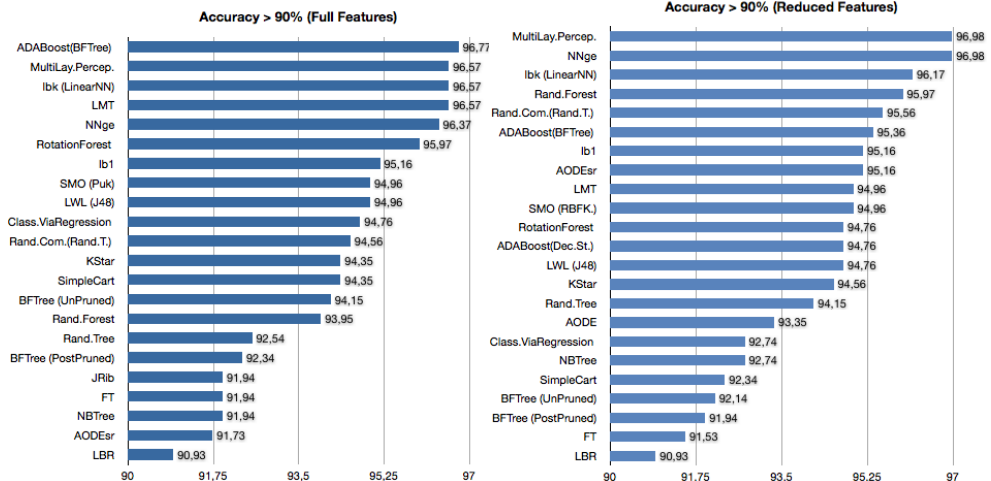
\includegraphics[width=\textwidth]{accuracy.png}
\caption{Preciznosti algoritama - sa svim atributima i bez}
\label{fig:acc}
\end{figure}

Na slici  \ref{fig:falsePos} se vidi isti trend kao i na slici  \ref{fig:acc}: smanjenjem broja atributa algoritmi zasnovani na stablima se losije ponasaju dok algoritmi najblizih suseda i ``MultiLayerPerceptron'' daju bolje rezultate.

\begin{figure}[h!]
\centering
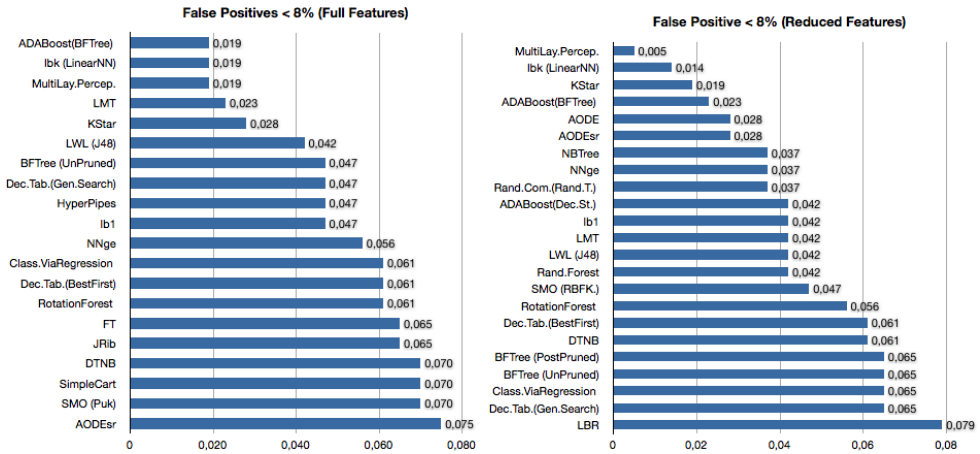
\includegraphics[width=\textwidth]{false_positive.png}
\caption{Lazni pozitivni - sa svim atributima i bez}
\label{fig:falsePos}
\end{figure}

%According to the results gained by Baca [3] it is very important for a static
%analysis tool to have a low false positive rate. According to that results if a tool
%signals to many false alarms the developer tend to ignore all signals or even worse,
%introduces new faults at the position the tool signals them

Prema rezultatima dobijenim u  \cite{baca} vrlo je bitno da alat staticke analize ima malo laznih pozitivnih jer
u slucaju mnogo pogresnih uzbuna razvijaoci pocinju da ignorisu te signali, ili jos gore izmenjuju ispravan kod sto dolazi 
do pravljenja novih greski kako bi izbegli upozorenja alata. Na slici \ref{fig:falseNeg} se vidi da je ``NNge'' najbolji, sto je i ocekivano s obzirom na prilicno 
lose performanse sto se tice laznih pozitivnih.

\begin{figure}[h!]
\centering
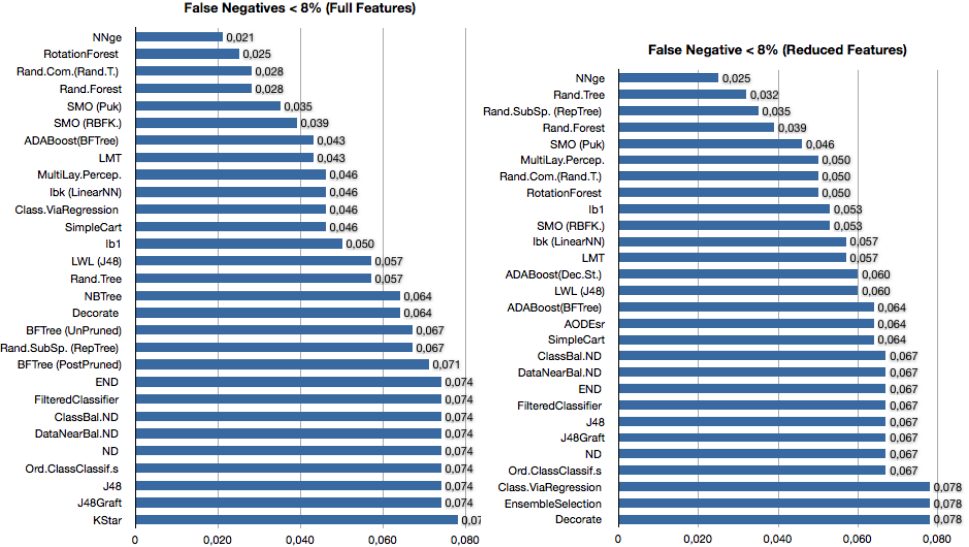
\includegraphics[width=\textwidth]{false_negative.png}
\caption{Lazni negativni - sa svim atributima i bez}
\label{fig:falseNeg}
\end{figure}




\subsection{... podnaslov}
\label{subsec:podnaslovM}

Ovde pišem tekst. 
Ovde pišem tekst. 
Ovde pišem tekst. 
Ovde pišem tekst. 
Ovde pišem tekst. 

\section{Poslednji naslov}
\label{sec:naslovM}

Ovde pišem tekst. 
Ovde pišem tekst. 
Ovde pišem tekst. 
Ovde pišem tekst. 
Ovde pišem tekst. 
Ovde pišem tekst. 
Ovde pišem tekst. 
Ovde pišem tekst. 
Ovde pišem tekst. 

\section{Zaključak}
\label{sec:zakljucak}

Ovde pišem zaključak. 
Ovde pišem zaključak. 
Ovde pišem zaključak. 
Ovde pišem zaključak. 
Ovde pišem zaključak. 
Ovde pišem zaključak. 
Ovde pišem zaključak. 
Ovde pišem zaključak. 
Ovde pišem zaključak. 
Ovde pišem zaključak. 
Ovde pišem zaključak. 
Ovde pišem zaključak. 


\addcontentsline{toc}{section}{Literatura}
\appendix
\bibliography{seminarski} 
\bibliographystyle{plain}



\end{document}
